\chapter{Projektplan}
\label{cha:projektplan}

Das Arbeiten in einem Team, indem es keine Hierarchie geben soll, ist verbunden mit agilem Entwickeln. Wichtig f"ur keine strenge Rolleneinteilungen ist die permanente Dokumentation und das verständliche Entwickeln, damit die Weiterentwicklung von allen Teammitgliedern zu jeder Zeit möglich ist. Die Kommunikation der Mitglieder und der Austausch von neu erlerntem Wissen funktionierten azyklisch. Terminierte Treffen wurden einberufen um unsere Fortschritte zu besprechen und neue Anforderungen des Projektbetreuers zu bekommen. Einen Zeitplan mit einigen Meilensteine, haben wir nach der ersten Einarbeitungsphase erstellt. Anhand von diesem können wir gut unsere Fortschritte und unsere Misserfolge darstellen. Die Anpassung der Zwischenschritte wird in Kapitel Probleme genauer dargestellt.\newline
Die Abbildung \ref{ms1} zeigt den genaueren Zeitplan, mit mehreren Arbeitspaketen, welche einen Zeiteinschätzung haben und an denen man erkennen kann welche Pakete von welchen Abhängen. Die Zwischenziele sind als Meilensteine aufgetragen. Das erfolgreiche Abschließen der Arbeitspakete und Meilensteine wurde bis zum Zwischentermin abgeschlossen. Die Einarbeitungsphase und die Lieferung der Hardware haben viel Zeit eingenommen, werden aber nicht weiter thematisiert. Bis zur Zwischenpräsentation sollten das wichtige Arbeitspaket der Kamerakalibrierung abgeschlossen sein. Des Weiteren sollte die Generierung der Punktewolke stattfinden

\begin{figure}[H]
	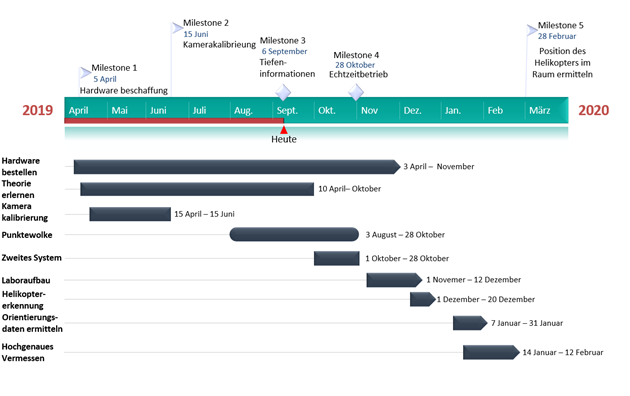
\includegraphics[scale=0.36]{bilder/ms1}
	\caption[Projektplan Zwischenergebnis]{Projektplan Zwischenergebnis}
	\label{fig:ms1}
\end{figure}

\noindent In dem endgültigen Plan mussten einige Anpassungen getroffen werden. Dies ist in der Abbildung \ref{fig:ms2} rot markiert. Der nicht eingehaltene Meilenstein 4: Echtzeitbetrieb, wurde vorerst verschoben und dann als nicht relevant für die Aufgabenstellung und die Algorithmus Entwicklung beschlossen. Das Arbeitspaket Kamerakalibrierung hat sich sehr in die Länge gezogen und ist auch noch präsent bei dem Abschluss des Projektes. Sie führt immer wieder zu Ungenauigkeiten und wird im Kapitel Probleme behandelt. Das Arbeitspaket Orientierungsdaten ermitteln, wurde in der Art geändert, dass der Helikopter erkannt wird aber nicht in seiner Ausrichtung im Raum. Die Bearbeitung nach unserem Projektplan hat zu einem Ergebnis geführt, das in den nächsten Kapiteln dargestellt wird. 

\begin{figure}[H]
	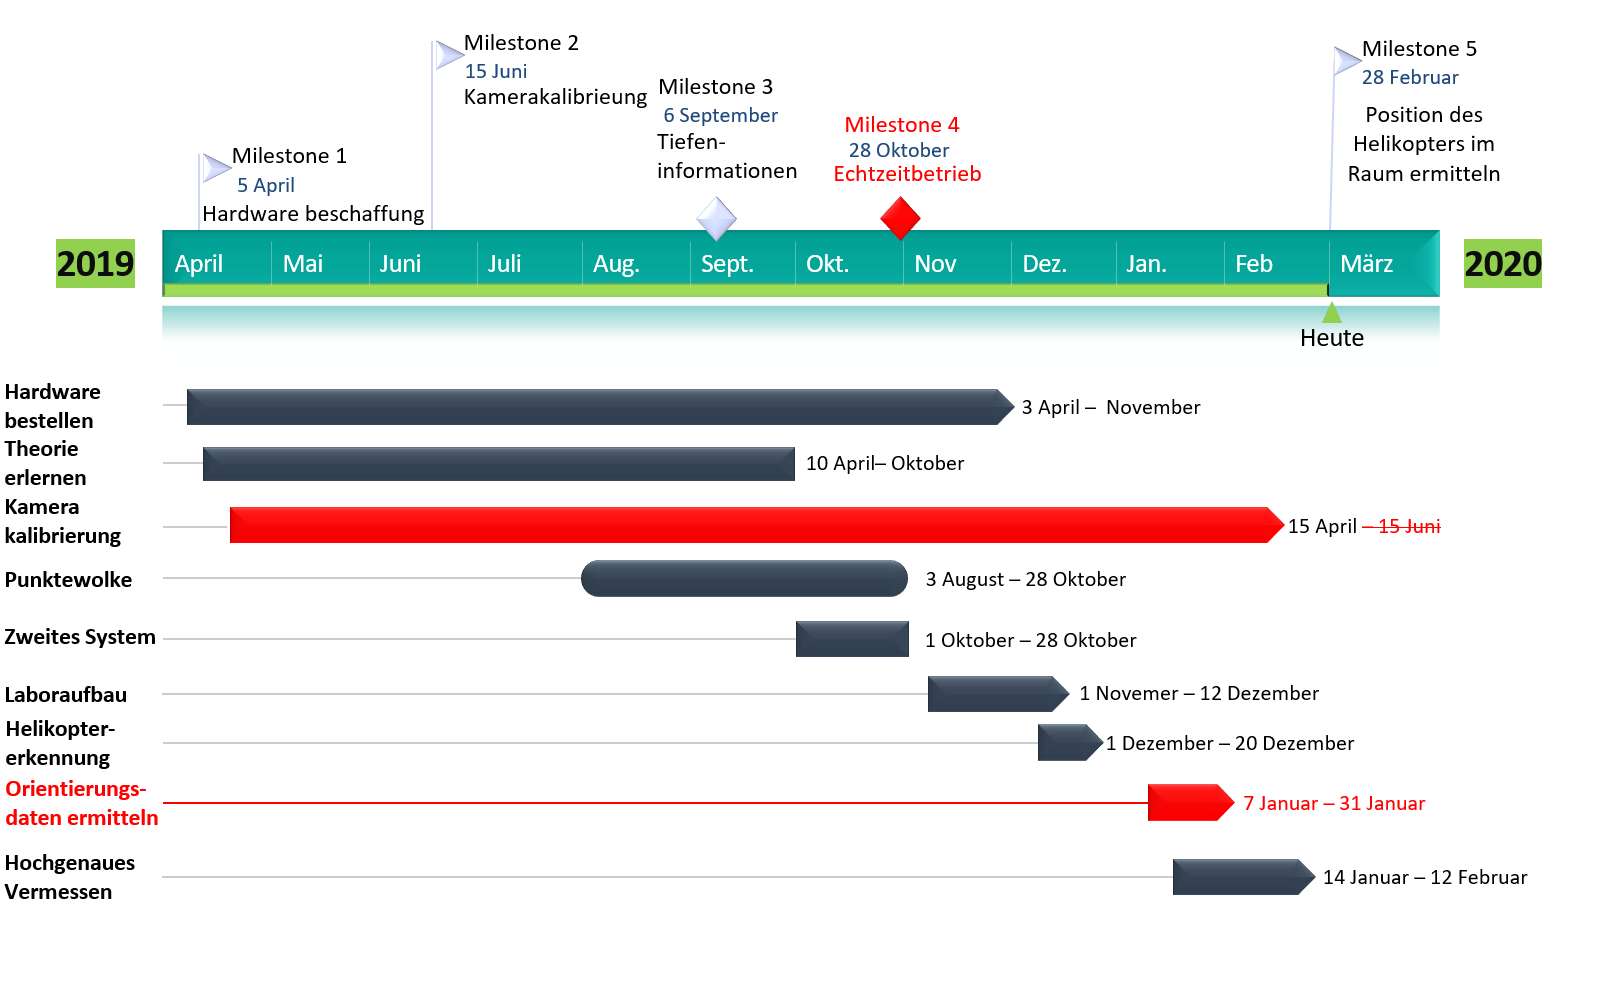
\includegraphics[scale=0.36]{bilder/ms2}
	\caption[Endgültiger Zeitplan ]{Endgültiger Zeitplan }
	\label{fig:ms2}
\end{figure}